\documentclass[12pt]{jarticle}
\usepackage{TUSIReport}
\usepackage{otf}
\usepackage{ascmac}
\usepackage{listings,jlisting}
\usepackage{url}
\usepackage[dvipdfmx]{graphicx}
\usepackage{here}
\usepackage{subfigure}
\usepackage{amssymb}
\usepackage{multirow}
\usepackage{longtable}
\setlength{\textwidth}{170mm}       % テキストの幅
\setlength{\textheight}{260mm}      % テキストの高さ
\setlength{\oddsidemargin}{-5mm}    % 偶数ページの左マージン
\setlength{\evensidemargin}{0mm}    % 奇数ページの左マージン
\setlength{\topmargin}{-25mm}       % 上のマージン  % 奇数ページの左マージン
\lstset{
  basicstyle={\ttfamily},
  identifierstyle={\small},
  commentstyle={\smallitshape},
  keywordstyle={\small\bfseries},
  ndkeywordstyle={\small},
  stringstyle={\small\ttfamily},
  frame={tb},
  breaklines=true,
  columns=[l]{fullflexible},
  numbers=left,
  xrightmargin=0zw,
  xleftmargin=3zw,
  numberstyle={\scriptsize},
  stepnumber=1,
  numbersep=1zw,
  lineskip=-0.5ex
}
\begin{document}
%%%%%%%%%%%%%%%%%%%%%%%%%%%%%%%%%%%%%%%%%%%%%%%%%%%%%%%%%%%%%%
% 表紙を出力する場合は,\提出者と\共同実験者をいれる
% \提出者{科目名}{課題名}{提出年}{提出月}{提出日}{学籍番号}{氏名}
% \共同実験者{一人目}{二人目}{..}{..}{..}{..}{..}{八人目}
%%%%%%%%%%%%%%%%%%%%%%%%%%%%%%%%%%%%%%%%%%%%%%%%%%%%%%%%%%%%%%
\提出者{情報工学実験2}{実験テーマ3 情報通信シミュレーション}{2020}{10}{12}{4619023}{加藤零}
\共同実験者{\large{}}{\large{}}{\large{}}{\large{}}{\large{}}{\large{}}{\large{}}{}

%%%%%%%%%%%%%%%%%%%%%%%%%%%%%%%%%%%%%%%%%%%%%%%%%%%%%%%%%%%%%%
% 表紙を出力しない場合は,以下の「\表紙出力」をコメントアウトする
%%%%%%%%%%%%%%%%%%%%%%%%%%%%%%%%%%%%%%%%%%%%%%%%%%%%%%%%%%%%%%
\表紙出力

%%%%%%%%%%%%%%%%%%%%%%%%%%%%%%%%%%%%%%%%%%%%%%%%%%%%%%%%%%%%%%
% 以下はレポート本体である.別途 TeXファイルを作成し \input 使っても良い
%%%%%%%%%%%%%%%%%%%%%%%%%%%%%%%%%%%%%%%%%%%%%%%%%%%%%%%%%%%%%%

\section{実験}
$\epsilon$の値とそれに対応するビット誤り率$P_e$を$\rm{MT}$()及び$\rm{rand()}$を利用して生成した乱数を使用してシミュレーションする.ソースコードは全て付録に記載した.

\section{実験環境}
以下の環境下で課題に取り組んだ..
\begin{itemize}
    \item OS: macOS Catalina バージョン 10.15.7
    \item CPU: Intel Core i5 2.4 GHz クアッドコア
    \item clang: Apple clang version 12.0.0 (clang-1200.0.32.2)
\end{itemize}

\section{結果}
\begin{itemize}
    \item $\epsilon=0.0001$として,シミュレーション回数SIMを変化させると表1,2,3のような結果を得られた.また,それらをグラフにプロットしたところ図1,2,3のようになった.
\end{itemize}
\begin{table}[h]
    \begin{minipage}{0.5\hsize}
        \begin{center}
            \caption{SIM=10000の時の結果}
            \begin{tabular}{|r|r|r|} \hline
                \multicolumn{1}{|c|}{理論値} & \multicolumn{1}{|c|}{rand()} & \multicolumn{1}{|c|}{MT} \\\hline
                0.0001                       & 0.000075                     & 0.000075                 \\\hline
                0.0002                       & 0.000125                     & 0.000100                 \\\hline
                0.0003                       & 0.000325                     & 0.000325                 \\\hline
                0.0004                       & 0.000350                     & 0.000350                 \\\hline
                0.0005                       & 0.000525                     & 0.000650                 \\\hline
                0.0006                       & 0.000525                     & 0.000875                 \\\hline
                0.0007                       & 0.000800                     & 0.000750                 \\\hline
                0.0008                       & 0.000675                     & 0.000950                 \\\hline
                0.0009                       & 0.000725                     & 0.000775                 \\\hline
                0.0010                       & 0.001075                     & 0.000950                 \\\hline
            \end{tabular}
        \end{center}
    \end{minipage}
    \begin{minipage}{0.5\hsize}
        \begin{center}
            \caption{SIM=100000の時の結果}
            \begin{tabular}{|r|r|r|} \hline
                \multicolumn{1}{|c|}{理論値} & \multicolumn{1}{|c|}{rand()} & \multicolumn{1}{|c|}{MT} \\\hline
                0.0001                       & 0.0000875                    & 0.0000950                \\\hline
                0.0002                       & 0.0002075                    & 0.0002275                \\\hline
                0.0003                       & 0.0002700                    & 0.0003175                \\\hline
                0.0004                       & 0.0003675                    & 0.0004575                \\\hline
                0.0005                       & 0.0004400                    & 0.0005375                \\\hline
                0.0006                       & 0.0005750                    & 0.0005825                \\\hline
                0.0007                       & 0.0006925                    & 0.0006850                \\\hline
                0.0008                       & 0.0007800                    & 0.0007825                \\\hline
                0.0009                       & 0.0008675                    & 0.0008775                \\\hline
                0.0010                       & 0.0010050                    & 0.0009500                \\\hline
            \end{tabular}
        \end{center}
    \end{minipage}
\end{table}
\clearpage
\begin{table}[h]
    \begin{minipage}{0.5\hsize}
        \begin{center}
            \caption{SIM=1000000の時の結果}
            \begin{tabular}{|r|r|r|} \hline
                \multicolumn{1}{|c|}{理論値} & \multicolumn{1}{|c|}{rand()} & \multicolumn{1}{|c|}{MT} \\\hline
                0.0001                       & 0.00009080                   & 0.0000995                \\\hline
                0.0002                       & 0.00019425                   & 0.0002105                \\\hline
                0.0003                       & 0.00030225                   & 0.0002985                \\\hline
                0.0004                       & 0.00041225                   & 0.0004013                \\\hline
                0.0005                       & 0.00049675                   & 0.0005085                \\\hline
                0.0006                       & 0.00059475                   & 0.0006153                \\\hline
                0.0007                       & 0.00071375                   & 0.0007213                \\\hline
                0.0008                       & 0.00080100                   & 0.0007690                \\\hline
                0.0009                       & 0.00089575                   & 0.0008800                \\\hline
                0.0010                       & 0.00099650                   & 0.0009990                \\\hline
            \end{tabular}
        \end{center}
    \end{minipage}
\end{table}
\begin{figure}[H]
    \begin{center}
        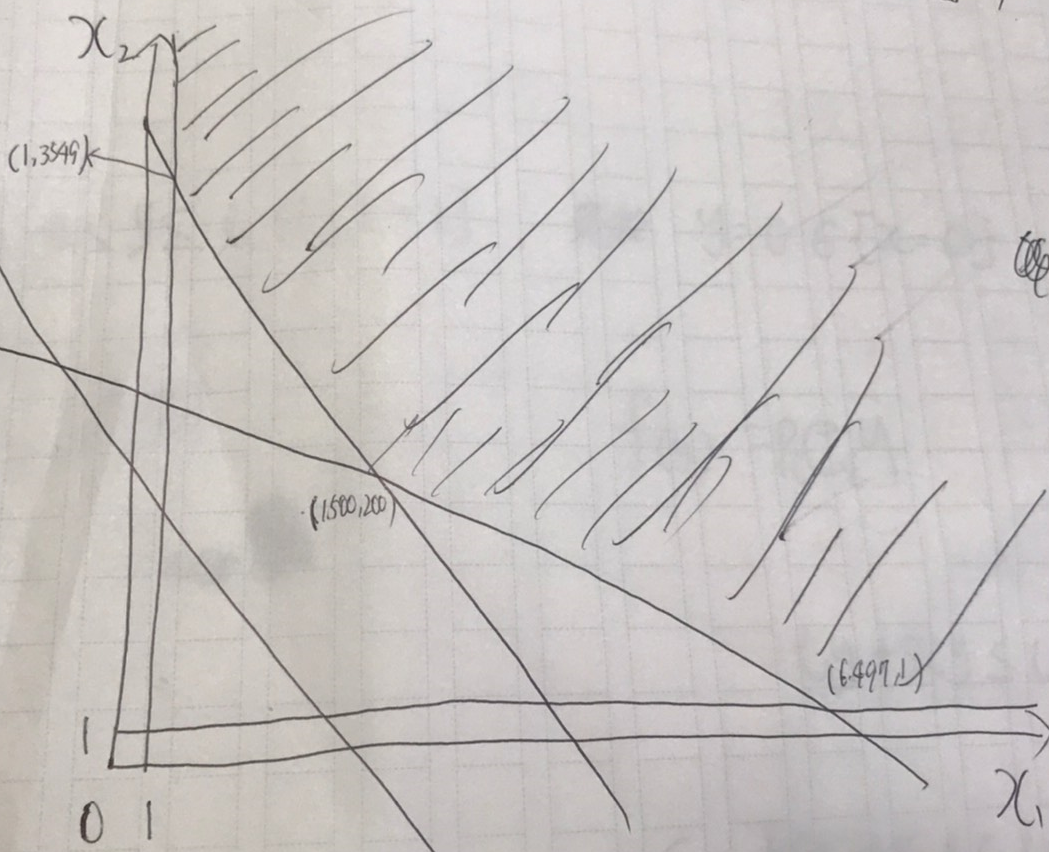
\includegraphics[bb=0 0 332 217,height=6cm]{1.png}
    \end{center}
    \caption{SIM=10000の時のビット誤り率の推移}
    \label{fig1}
\end{figure}
\begin{figure}[H]
    \begin{center}
        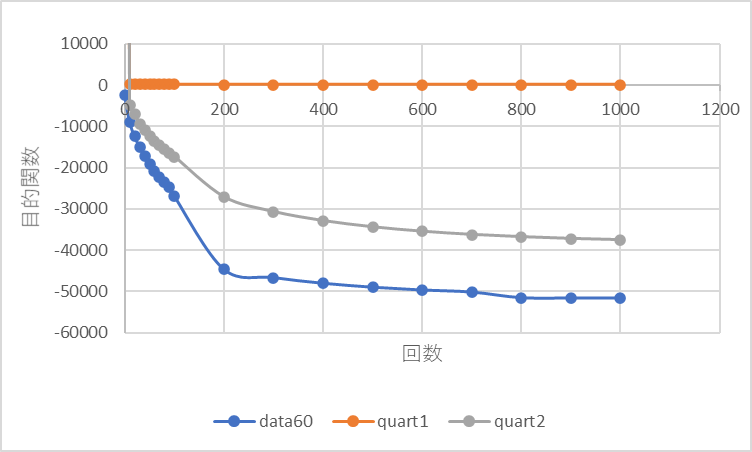
\includegraphics[bb=0 0 332 217,height=6cm]{2.png}
    \end{center}
    \caption{SIM=100000の時のビット誤り率の推移}
    \label{fig1}
\end{figure}
\begin{figure}[H]
    \begin{center}
        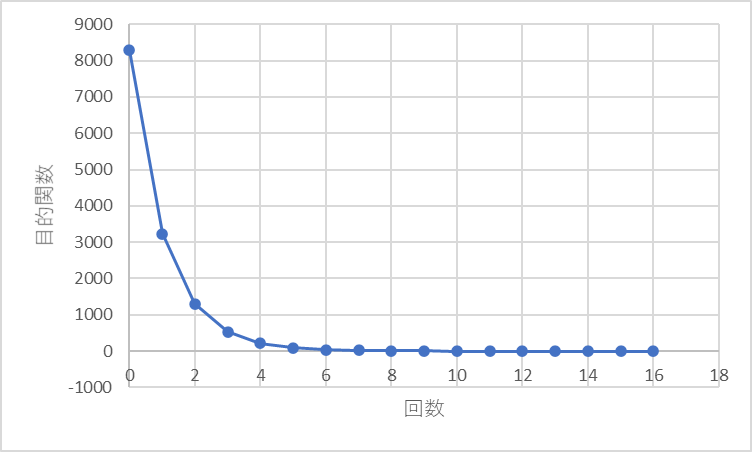
\includegraphics[bb=0 0 332 217,height=6cm]{3.png}
    \end{center}
    \caption{SIM=1000000の時のビット誤り率の推移}
    \label{fig1}
\end{figure}
\begin{itemize}
    \item シミュレーション回数SIMを100000に固定したまま$\epsilon$を変化させると表4,5のような結果を得られた.また,それらをグラフにプロットしたところ図4,5のようになった.
\end{itemize}
\begin{table}[h]
    \begin{minipage}{0.5\hsize}
        \begin{center}
            \caption{$\epsilon=0.00001$の時の結果}
            \begin{tabular}{|r|r|r|} \hline
                \multicolumn{1}{|c|}{理論値} & \multicolumn{1}{|c|}{rand()} & \multicolumn{1}{|c|}{MT} \\\hline
                0.00001                      & 0.0000025                    & 0.0000050                \\\hline
                0.00002                      & 0.0000200                    & 0.0000150                \\\hline
                0.00003                      & 0.0000375                    & 0.0000450                \\\hline
                0.00004                      & 0.0000325                    & 0.0000475                \\\hline
                0.00005                      & 0.0000450                    & 0.0000575                \\\hline
                0.00006                      & 0.0000725                    & 0.0000700                \\\hline
                0.00007                      & 0.0000750                    & 0.0000475                \\\hline
                0.00008                      & 0.0000550                    & 0.0000575                \\\hline
                0.00009                      & 0.0000750                    & 0.0001075                \\\hline
                0.00010                      & 0.0000950                    & 0.0000900                \\\hline
            \end{tabular}
        \end{center}
    \end{minipage}
    \begin{minipage}{0.5\hsize}
        \begin{center}
            \caption{$\epsilon=0.001$の時の結果}
            \begin{tabular}{|r|r|r|} \hline
                \multicolumn{1}{|c|}{理論値} & \multicolumn{1}{|c|}{rand()} & \multicolumn{1}{|c|}{MT} \\\hline
                0.001                        & 0.0009950                    & 0.0010300                \\\hline
                0.002                        & 0.0019250                    & 0.0019875                \\\hline
                0.003                        & 0.0031400                    & 0.0029975                \\\hline
                0.004                        & 0.0039350                    & 0.0041775                \\\hline
                0.005                        & 0.0050300                    & 0.0050225                \\\hline
                0.006                        & 0.0060250                    & 0.0060550                \\\hline
                0.007                        & 0.0073400                    & 0.0069450                \\\hline
                0.008                        & 0.0078650                    & 0.0077950                \\\hline
                0.009                        & 0.0089775                    & 0.0089525                \\\hline
                0.010                        & 0.0098925                    & 0.0099375                \\\hline
            \end{tabular}
        \end{center}
    \end{minipage}
\end{table}
\begin{figure}[H]
    \begin{center}
        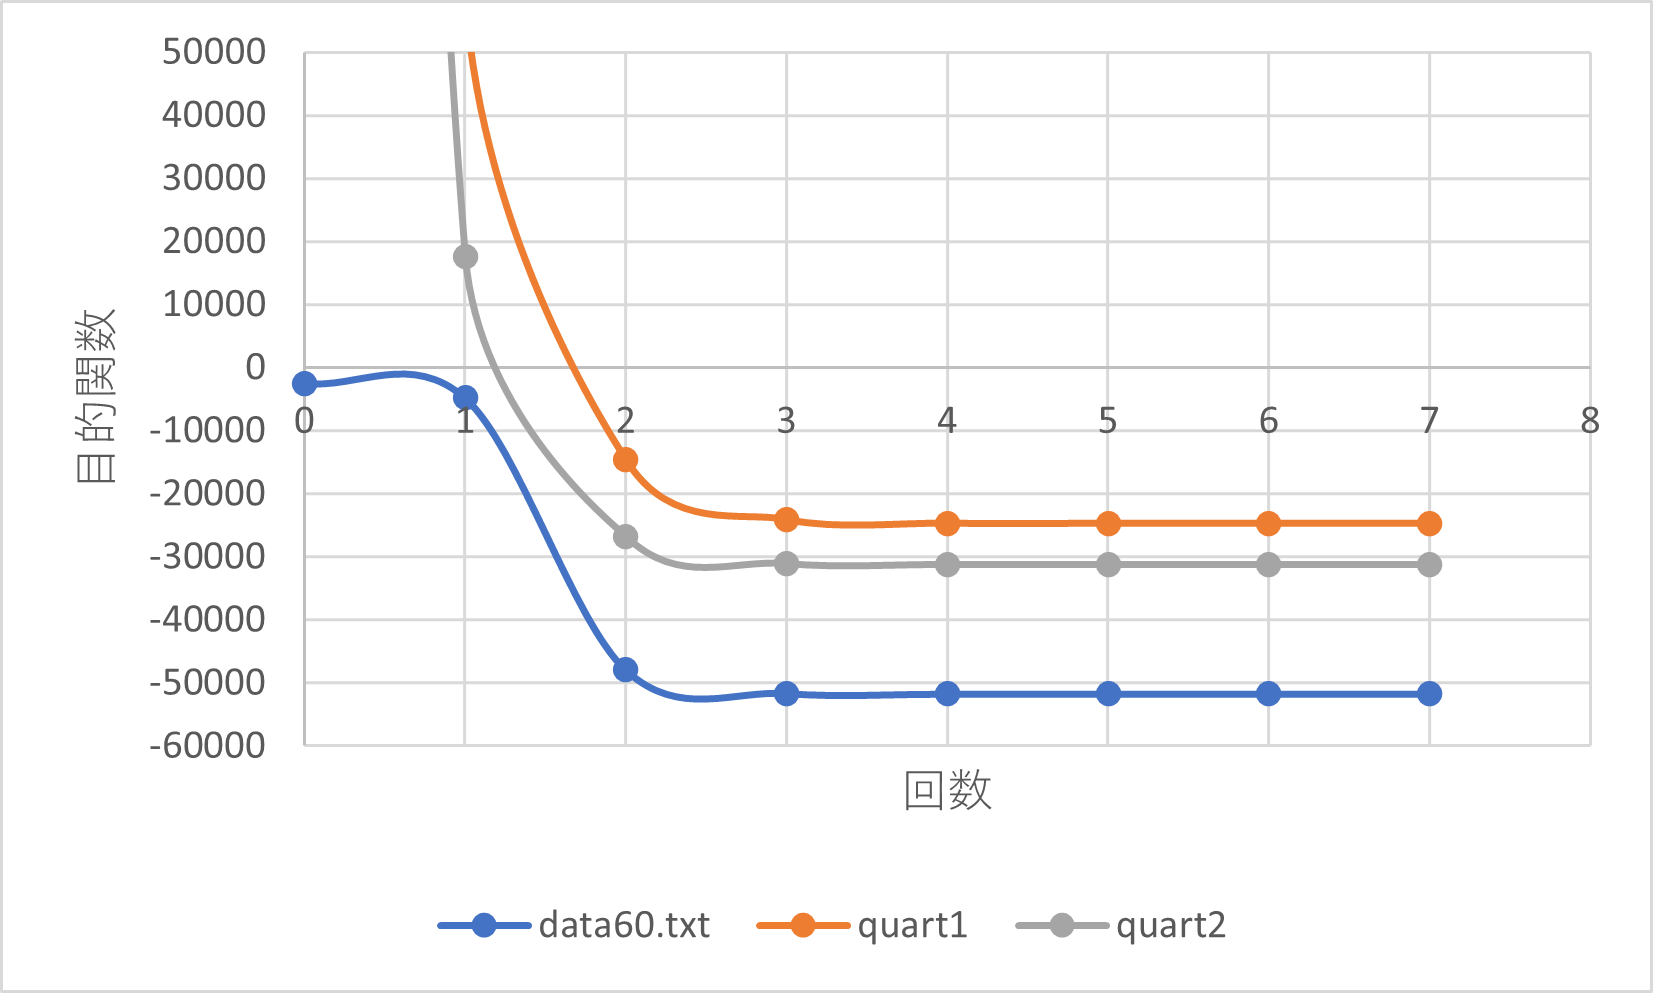
\includegraphics[bb=0 0 332 217,height=6cm]{4.png}
    \end{center}
    \caption{$\epsilon=0.00001$の時のビット誤り率の推移}
    \label{fig1}
\end{figure}
\begin{figure}[H]
    \begin{center}
        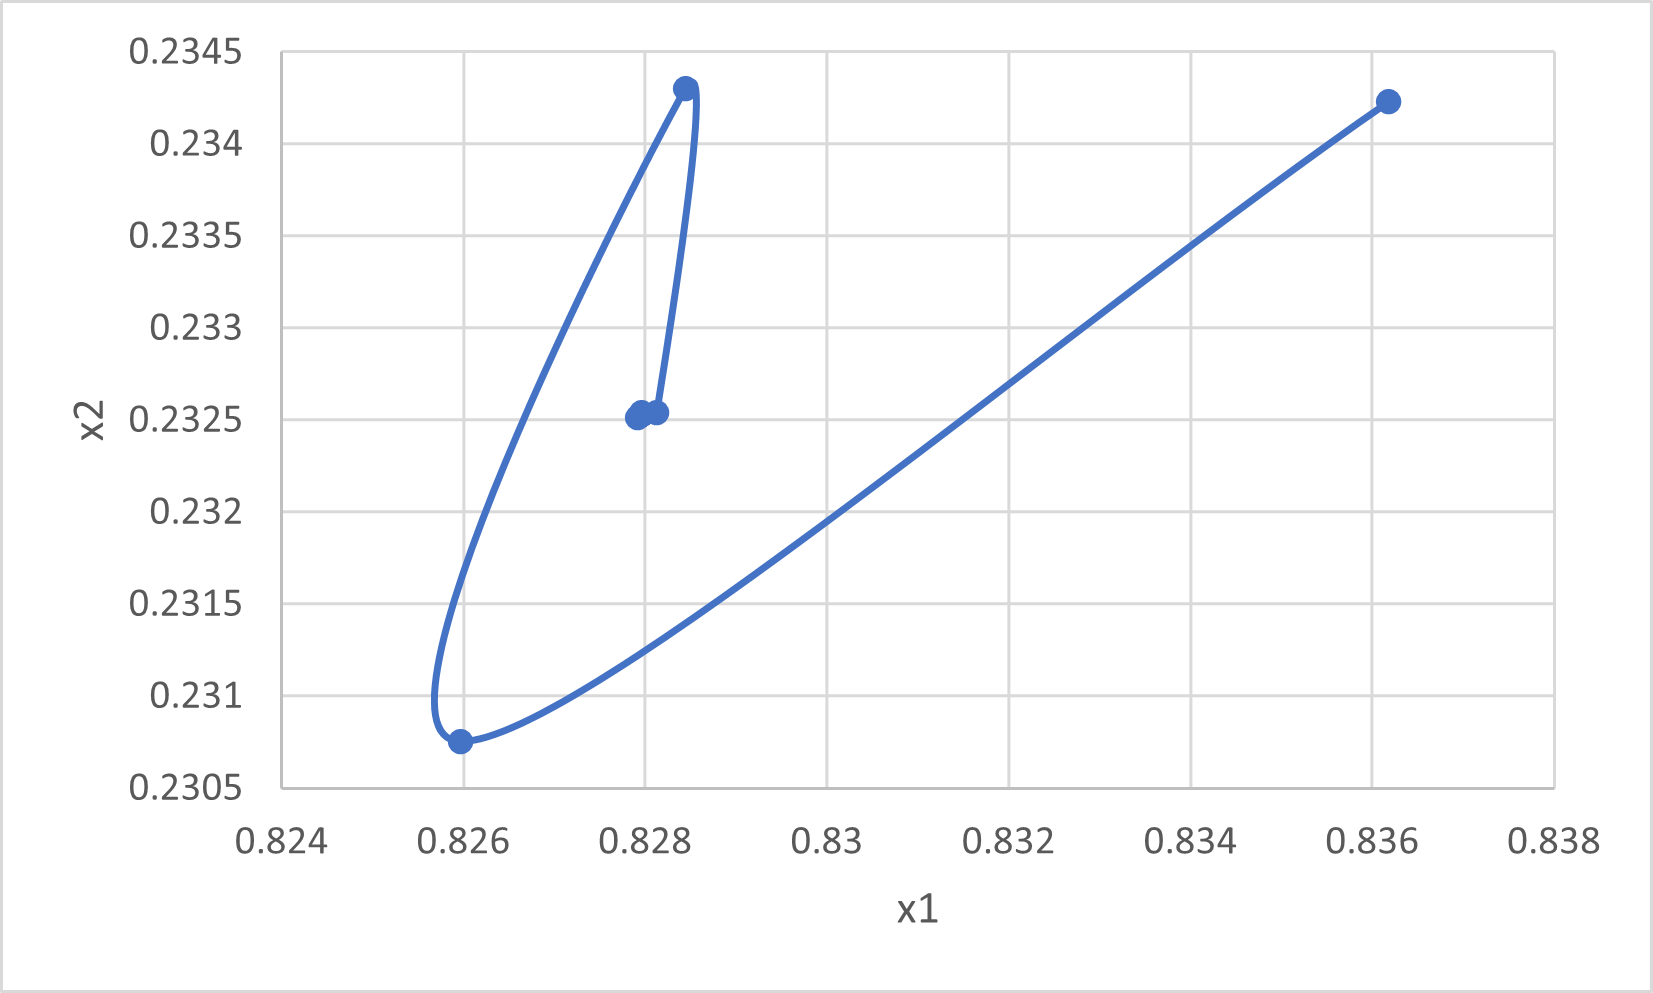
\includegraphics[bb=0 0 332 217,height=6cm]{5.png}
    \end{center}
    \caption{$\epsilon=0.001$の時のビット誤り率の推移}
    \label{fig1}
\end{figure}
\section{検討事項}
\subsection{課題1-1}
\begin{shadebox}
    \quad シミュレーションによるビット誤り率と理論値がほぼ同じ値になるにはどの程度のシミュレーション回数を実行する必要があるか.
\end{shadebox}
\vspace{\baselineskip}
図1,2,3に着目するとシミュレーション回数を増やすほど誤差が小さくなっていることがわかる.図1の条件の下,理論値と実験値の相対誤差の平均をとると$\rm{rand()}$は約15.8\%,$\rm{MT}$は約21.6\%となる.同様に図2では$\rm{rand()}$が約5.82\%,$\rm{MT}$が約6.12\%となり,図3では$\rm{rand()}$が約2.04\%,$\rm{MT}$が約2.00\%となる.実際にソースコード3,4を利用してシミュレーション回数を変化した場合の相対誤差を計測した結果をグラフにプロットしたところ,図6のようになった.対数の法則よりシミュレーション回数を増やすことで理論値との相対誤差の平均は減少していくことがわかるが,図6のグラフの終端あたりでは振動している.このことから,相対誤差を1\%以下にするためには膨大なシミュレーション回数が必要となる.グラフに着目すると,800000回あたりで変動が小さくなるため,この辺りが理論値に近しくなるといえる.また,今回のソースコード3の実行速度は4に比べて高速であったことから,$\rm{rand()}$を用いた方が$\rm{MT}$より高速に乱数を生成できることがわかった.
\begin{figure}[H]
    \begin{center}
        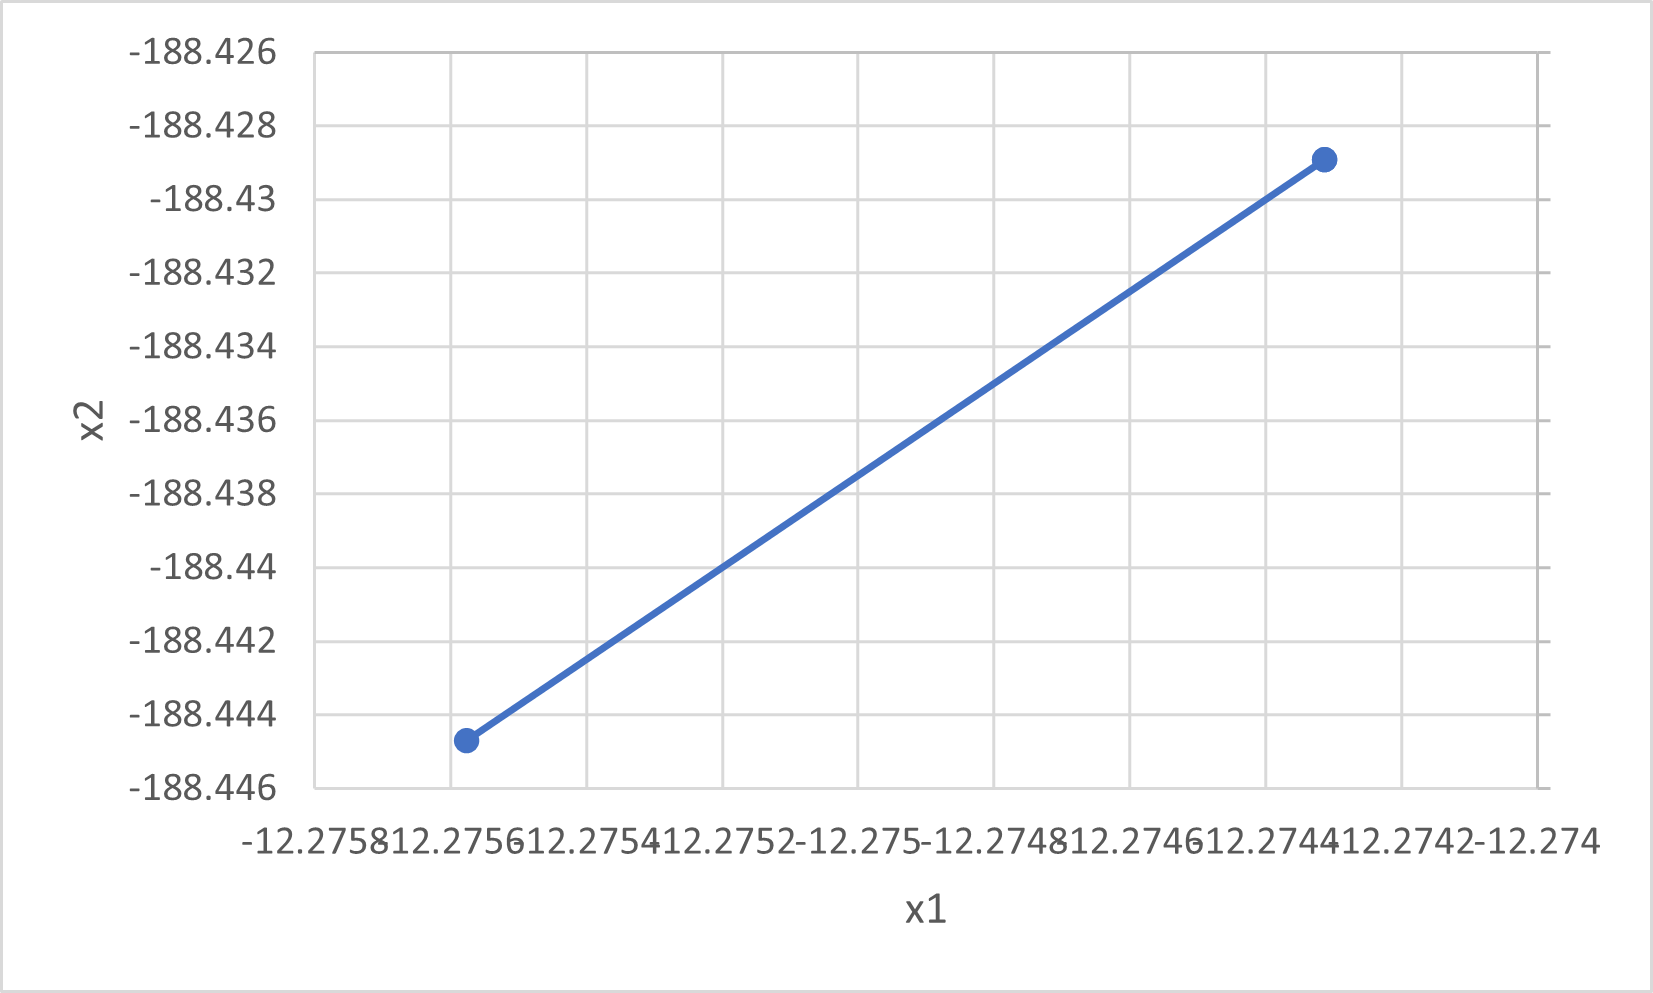
\includegraphics[bb=0 0 412 217,height=6cm]{6.png}
    \end{center}
    \caption{シミュレーション回数を変化させた時の相対誤差の平均値の推移($\epsilon=0.0001$)}
    \label{fig1}
\end{figure}
\subsection{課題1-2}
\begin{shadebox}
    \quad $\epsilon$を非常に小さくした場合,これはどうなるか
\end{shadebox}
\vspace{\baselineskip}
課題1-1と同様に相対誤差の平均を用いて図4について考える.なお,$\epsilon=0.00001$とする.シミュレーション回数が10000回の時$\rm{rand()}$の相対誤差の平均は約59.6\%,$\rm{MT}$の相対誤差の平均は約45.6\%となる.シミュレーション回数が10000回の時だけに着目しても明らかに誤差が広がっている.課題1-1と同様にシミュレーション回数を変化させてグラフにプロットしたところ図7のようになった.図7に着目すると課題1-1のとき,すなわち$\epsilon=0.0001$の時と比べて相対誤差の平均が全体的に高くなっており,約10\%あたりに収束しているように読み取れる.以上より,$\epsilon$を小さくすると理論値と実験値が離れることがわかる.実際,図5において$\epsilon$を大きくした場合は理論値と実験値との差が小さくなっている.しかし,$\epsilon>0.5$となれば$\epsilon$と$1-\epsilon$の大小関係が反転するため再び誤差が大きくなると考えられる.
\begin{figure}[H]
    \begin{center}
        \includegraphics[bb=0 0 412 217,height=6cm]{7.png}
    \end{center}
    \caption{シミュレーション回数を変化させた時の相対誤差の平均値の推移($\epsilon=0.00001$)}
    \label{fig1}
\end{figure}
\subsection{課題1-3}
\begin{shadebox}
    \quad $\rm{rand()}$と$\rm{MT}$の違いは何か.
\end{shadebox}
\vspace{\baselineskip}
乱数とは過去のデータから予測できない値であり,ランダムな値である.しかし,コンピュータはプログラムにより構築されており,プログラムはアルゴリズムにより構築されている.アルゴリズムは決定論的であるため厳密な乱数をコンピュータ上で生成するのは不可能である。そのため,コンピュータは乱数生成のためのアルゴリズムを用いて擬似乱数を生成している.$\rm{rand()}$は線形合同法により構築されており,線形合同法とは定数$a,b,c$を用意して$x_{i+1}=ax_i+b \rm{mod} m$の漸化式を用いることで乱数を生成する方法である.この手法はMersenne Twisterの手法に比べて周期が短いため,多くの乱数を生成した場合に規則性が現れてしまう.上記の実験では図6,7のように$\rm{rand()}$と$\rm{MT}$にあまり違いが見られなかったが,$\epsilon=0.0001$として100000回,200000回,300000回$\cdots$10000000回のシミュレーションを行ったところ相対誤差の平均値は図8のようになった.このグラフの中央付近から終端にかけて$\rm{MT}$の方が$\rm{rand()}$より小さい値を取っていることがわかる.つまり,生成する乱数が多ければ多いほど$\rm{MT}$の方が$\rm{rand()}$より理論値に近づくといえる.また,このことから乱数の質は$\rm{MT}$の方が高いと言えるが,ソースコード4の実行速度はソースコード3の実行速度に比べ遅かったため,質よりも速度を優先する場合は$\rm{rand()}$を用いるのがよいと考えられる.
\begin{figure}[H]
    \begin{center}
        \includegraphics[bb=0 0 412 217,height=6cm]{8.png}
    \end{center}
    \caption{シミュレーション回数を変化させた時の相対誤差の平均値の推移($\epsilon=0.001,区間幅100000回$)}
    \label{fig1}
\end{figure}
\section{付録}
\begin{lstlisting}[title=ソースコード1,label=kadai1]
  #define _CRT_SECURE_NO_WARNINGS
  #include <stdio.h>
  
  #include <iomanip>
  #include <iostream>
  #include <random>
  using namespace std;
  #define SIM 100000
  #define rand (double)rand() / RAND_MAX;
  
  int main() {
      int K[4], Y[4], Noise[4];
      double eps = 0;
      srand(23);
      cout << "# SIM : " << SIM << "\n# ep # BER" << endl;
      for (int k = 0; k < 10; k++) {
          eps += 0.0001;
          int count = 0;
          for (int l = 0; l < SIM; l++) {
              for (int i = 0; i < 4; i++) {
                  double rnd = rand;
                  K[i] = rnd * 2;
              }
              for (int i = 0; i < 4; i++) {
                  double rnd = rand;
                  Noise[i] = rnd <= eps ? 1 : 0;
              }
              for (int i = 0; i < 4; i++) {
                  Y[i] = K[i] ^ Noise[i];
                  count += K[i] ^ Y[i];
              }
          }
          cout << eps << " " << (double)count / (4 * SIM) << endl;
      }
      return 0;
  }
  
\end{lstlisting}
\clearpage
\begin{lstlisting}[title=ソースコード2,label=kadai2]
  #define _CRT_SECURE_NO_WARNINGS
  #include <stdio.h>
  
  #include <iomanip>
  #include <iostream>
  #include <random>
  using namespace std;
  #define SIM 10000
  mt19937 mt(23);
  
  int main() {
      // [0,1]の小数を一様に発生させる       
      uniform_real_distribution<double> rand_real(0, 1);
      // 平均0,標準偏差0.3の正規分布に従う乱数
      normal_distribution<double> rand_n(0, 0.3);
      int K[4], Y[4], Noise[4];
      double eps = 0;
      cout << "# SIM : " << SIM << "\n# ep # BER" << endl;
      for (int k = 0; k < 10; k++) {
          eps += 0.0001;
          int count = 0;
          for (int l = 0; l < SIM; l++) {
              for (int i = 0; i < 4; i++) K[i] = rand_real(mt) * 2;
              for (int i = 0; i < 4; i++) Noise[i] = rand_real(mt) <= eps ? 1 : 0;
              for (int i = 0; i < 4; i++) {
                  Y[i] = K[i] ^ Noise[i];
                  count += K[i] ^ Y[i];
              }
          }
          cout << eps << " " << (double)count / (4 * SIM) << endl;
      }
      return 0;
  }
\end{lstlisting}
\clearpage
\begin{lstlisting}[title=ソースコード3,label=kadai3]
  #define _CRT_SECURE_NO_WARNINGS
  #include <stdio.h>
  
  #include <iomanip>
  #include <iostream>
  #include <random>
  using namespace std;
  #define rand (double)rand() / RAND_MAX;
  
  int SIM = 0;
  int main() {
      for (int i = 0; i < 100; i++) {
          srand(23);
          SIM += 10000;
          int K[4], Y[4], Noise[4];
          double eps = 0, diff = 0;
          for (int k = 0; k < 10; k++) {
              eps += 0.0001;
              int count = 0;
              for (int l = 0; l < SIM; l++) {
                  for (int i = 0; i < 4; i++) {
                      double rnd = rand;
                      K[i] = rnd * 2;
                  }
                  for (int i = 0; i < 4; i++) {
                      double rnd = rand;
                      Noise[i] = rnd <= eps ? 1 : 0;
                  }
                  for (int i = 0; i < 4; i++) {
                      Y[i] = K[i] ^ Noise[i];
                      count += K[i] ^ Y[i];
                  }
              }
              diff += abs((double)count / (4 * SIM) - eps) / 10 / eps;
          }
          cout << SIM << "相対誤差の平均:" << diff << endl;
      }
      return 0;
  }
  
\end{lstlisting}
\clearpage
\begin{lstlisting}[title=ソースコード4,label=kadai4]
  #define _CRT_SECURE_NO_WARNINGS
  #include <stdio.h>
  
  #include <iomanip>
  #include <iostream>
  #include <random>
  using namespace std;
  
  int SIM = 0;
  int main() {
      // [0,1]の小数を一様に発生させる       
      uniform_real_distribution<double> rand_real(0, 1);
      // 平均0,標準偏差0.3の正規分布に従う乱数
      normal_distribution<double> rand_n(0, 0.3);
      for (int i = 0; i < 100; i++) {
          mt19937 mt(23);
          SIM += 10000;
          int K[4], Y[4], Noise[4];
          double eps = 0, diff = 0;
          for (int k = 0; k < 10; k++) {
              eps += 0.0001;
              int count = 0;
              for (int l = 0; l < SIM; l++) {
                  for (int i = 0; i < 4; i++) K[i] = rand_real(mt) * 2;
                  for (int i = 0; i < 4; i++)
                      Noise[i] = rand_real(mt) <= eps ? 1 : 0;
                  for (int i = 0; i < 4; i++) {
                      Y[i] = K[i] ^ Noise[i];
                      count += K[i] ^ Y[i];
                  }
              }
              diff += abs((double)count / (4 * SIM) - eps) / 10 / eps;
          }
          cout << SIM << "相対誤差の平均:" << diff << endl;
      }
  
      return 0;
  }
\end{lstlisting}
% 参考文献
\begin{thebibliography}{99}
    \label{sannkoubunnkenn_chapter}
    \bibitem{} C言語による乱数生成\\
    \url{https://omitakahiro.github.io/random/random_variables_generation.html}\\
    最終閲覧日; 2020/10/18
\end{thebibliography}

%%%%%%%%%%%%%%%%%%%%%%%%%%%%%%%%%%%%%%%%%%%%%%%%%%%%%%%%%%%%%%
\end{document}